\begin{flushright} {\tiny {\color{gray} benchmark\_stokes\_sphere\_3D.tex}} \end{flushright}

\vspace{1cm}
\begin{flushright}
Data pertaining to this section are to be found at:
\url{https://github.com/cedrict/fieldstone/tree/master/images/stokes_sphere3D}
\end{flushright}
\vspace{1cm}

This is a simple experiment without an analytical solution. The idea here is simple: to design
a small number of Stokes sphere-related experiments and provide for them (very) high-resolution results 
obtained with various codes so as to turn these into benchmarks. 
The domain is chosen to be a unit cube. Gravity is such that $\vec{g}=(0,0,-g)$ with $g=1$. 
The sphere is in the middle of the domain and has a radius $R=0.123456798$.
The fluid has a density $\rho_f=1$ and viscosity $\eta_f=1$. The sphere has a density $\rho_s=\rho_f+\delta\rho$
and a viscosity $\eta_s=10^m \eta_f$. Default values for $\delta\rho$ and $m$ are 
set to 0.01 and 3 respectively.

Concerning boundary conditions, we distinguish three cases:
\begin{itemize}
\item FS: free slip boundary conditions are imposed on all 6 sides;
\item NS: no slip boundary conditions are imposed on all 6 sides;
\item OT: free slip boundary conditions are prescribed on the sides and bottom, but the top surface is open.
\item BO: both top and bottom are open (still with $u=0$) and no-slip is prescribed on the sides.
\end{itemize}

In the FS and NS case the null space of the pressure will need to be addressed and we require that the average 
pressure over the domain is zero, i.e.
\[
\iiint_\Omega p(x,y,z) dxdydx = 0
\]
The following quantities are reported:
\begin{itemize}
\item the root mean square velocity $\upnu_{rms}$ over the whole domain;
\item the minimum and maximum velocity and pressure in the domain (i.e. $u_{\text min,max}$, $v_{\text min,max}$,
      $w_{\text min,max}$ and $p_{\text min,max}$;
\item the velocity in the center of the sphere (maybe).
\end{itemize}

\noindent The factors which are expected to influence these measurements are:
\begin{itemize}
\item the resolution, especially if hexahedral elements are used;
\item the quadrature rule, especially if the material properties are directly prescribed on these;
\item the type of numerical method and their order (think $Q_1\times P_0$ vs $Q_2\times Q_1$ vs $Q_2 \times P_{-1}$
      vs ... for finite elements)
\item whether full or reduced densities are used (except for OT case);
\item the parameter $m$ which controls the rigidity of the sphere with regards to the surrounding fluid;
\item the relative density difference between the fluid and the sphere.
\end{itemize}

Stokes' law was derived by George Gabriel Stokes in 1851.  It describes the frictional force a sphere with
a density different than the surrounding fluid experiences in a laminar flowing viscous medium around it. 
By equating the frictional force term $6\pi \eta_f R \upnu_s$ with the buoyancy force $4/3 \pi R^3 \delta\rho g$, 
we arrive at the following settling velocity:
\[
\upnu_s = \frac{2}{9} \frac{\delta\rho R^2 g}{\eta_f}
\]
All the measurements above will then be adimensionalised by dividing all velocities by $\upnu_s$ and pressures
by $p_{ref}=\rho_f g L_z = 1$. Note that Stokes law is derived in an infinite fluid so that the recovered sphere 
velocity measurements are not expected to match this analytical value exactly.
In our case we have 
\[
\upnu_s = \frac29 \frac{0.01\cdot 0.123456789^2\cdot 1}{1} \simeq 0.00003387017 = 3.387017 \cdot 10^{-5}
\]

Note that as noted in the Gale manual\footnote{\url{https://geodynamics.org/cig/software/gale/}} 
a correction can be made
to this velocity when the sphere is itself viscous, see problem 2 p65-66
of second English edition of 'Fluid Mechanics' by Landau \& Lifshitz, volume 6
of Theoretical Physics.  


\newpage
\begin{center}
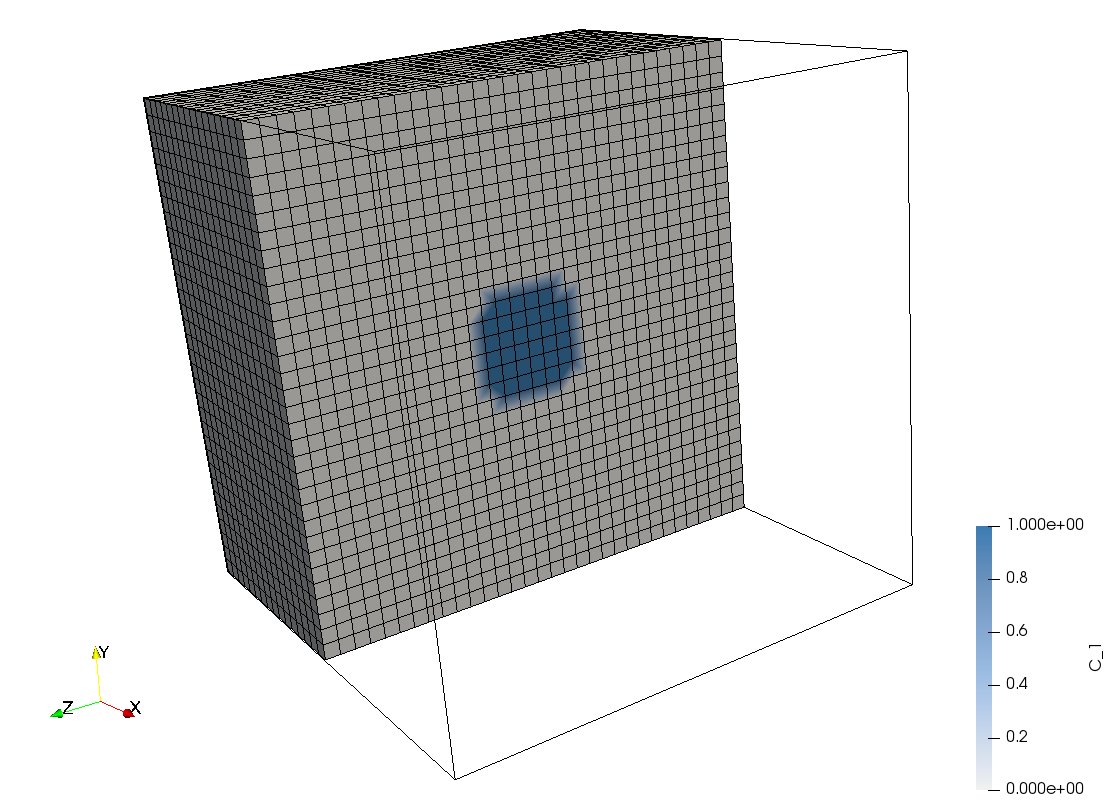
\includegraphics[width=5cm]{images/stokes_sphere3D/aspect_amr_FS/C1_0}
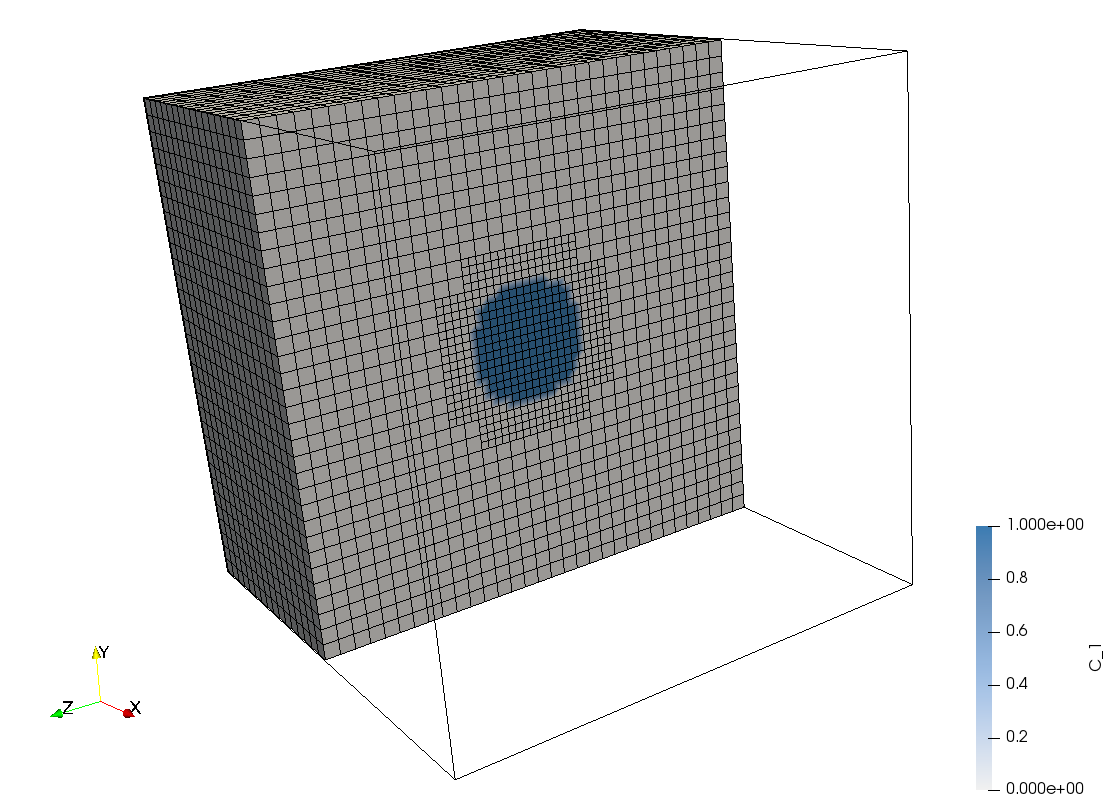
\includegraphics[width=5cm]{images/stokes_sphere3D/aspect_amr_FS/C1_1}
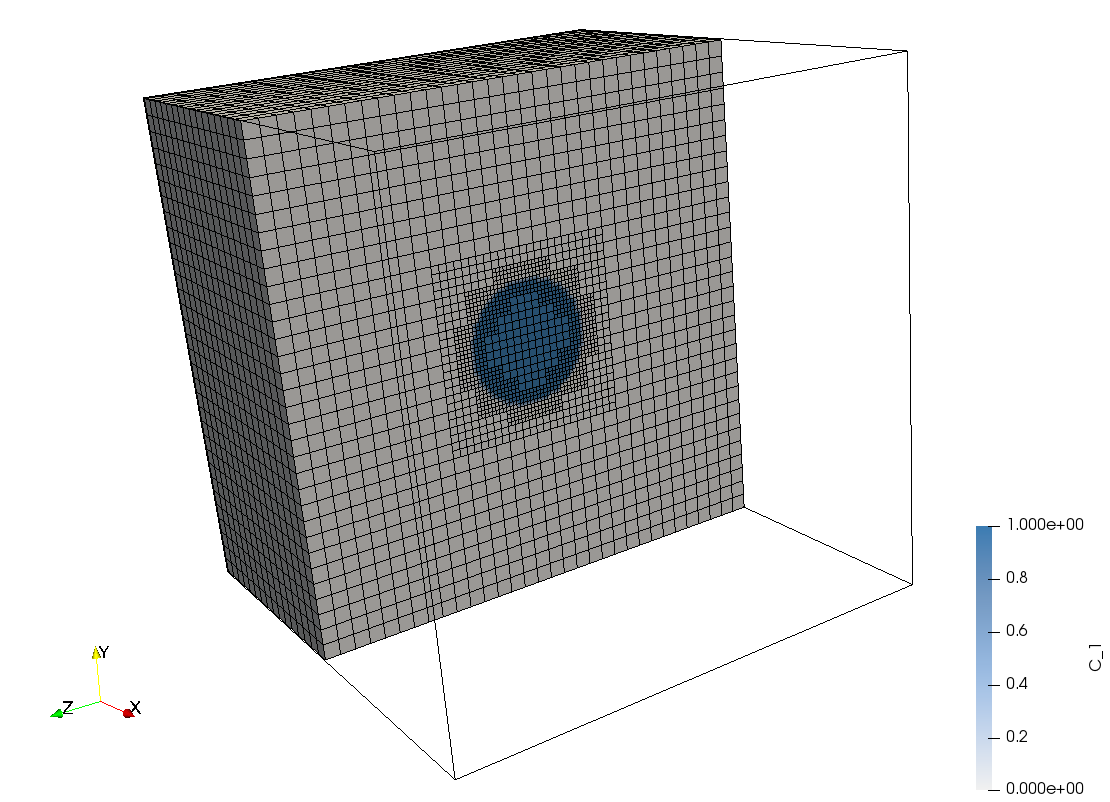
\includegraphics[width=5cm]{images/stokes_sphere3D/aspect_amr_FS/C1_2}\\
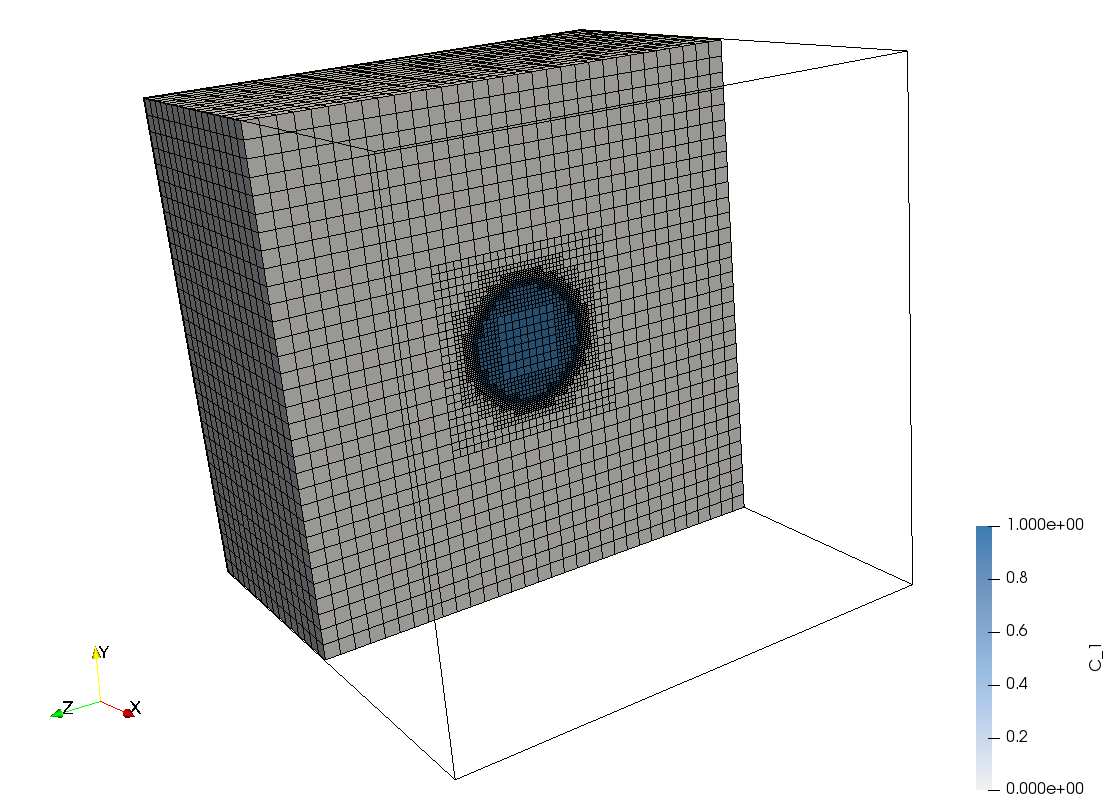
\includegraphics[width=5cm]{images/stokes_sphere3D/aspect_amr_FS/C1_3}
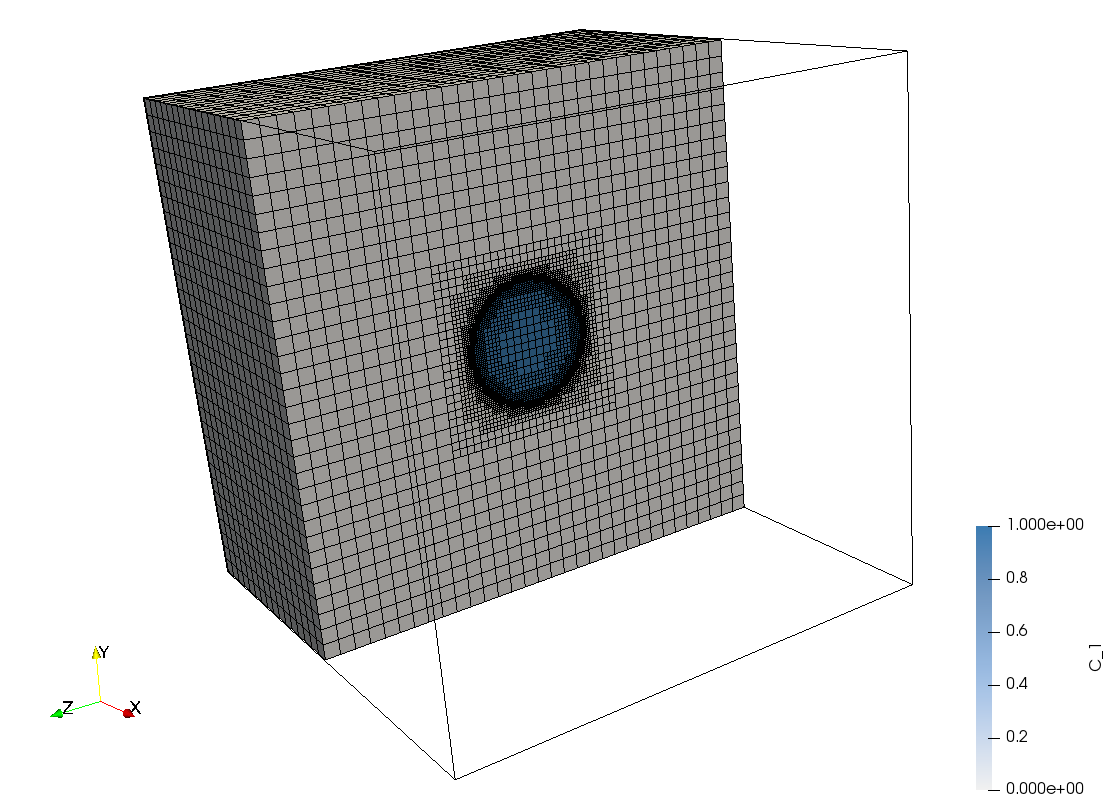
\includegraphics[width=5cm]{images/stokes_sphere3D/aspect_amr_FS/C1_4}\\
{\captionfont Octree-based \aspect meshes. The background mesh is $16^3$ and refinement is allowed to take place 4 times.
Note that a special output is automatically generated in the code which subdivides all elements in 8 for 
visualisation purposes only.}
\end{center}


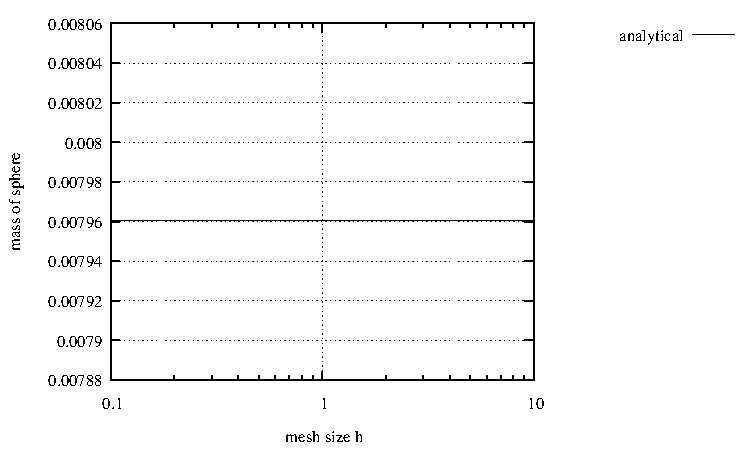
\includegraphics[width=7cm]{images/stokes_sphere3D/mass_sphere}
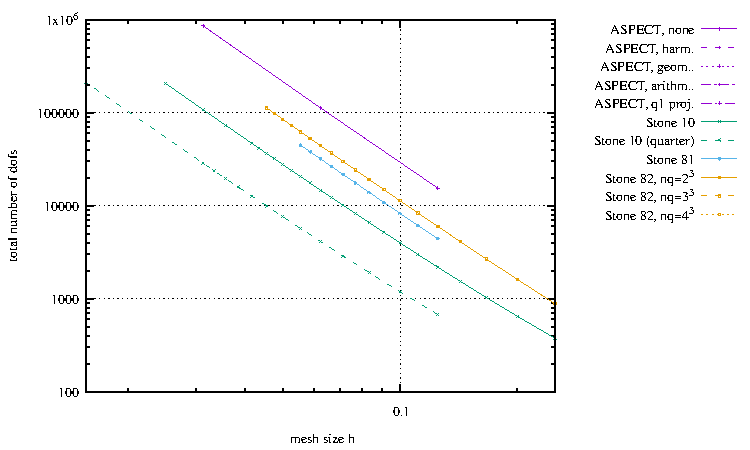
\includegraphics[width=7cm]{images/stokes_sphere3D/dofs}

\newpage
%.................................................................................
\paragraph{FS results}

\begin{center}
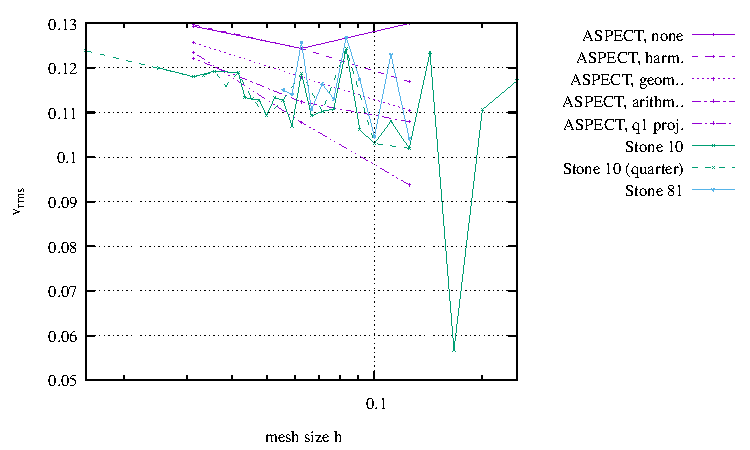
\includegraphics[width=5cm]{images/stokes_sphere3D/vrms_FS}
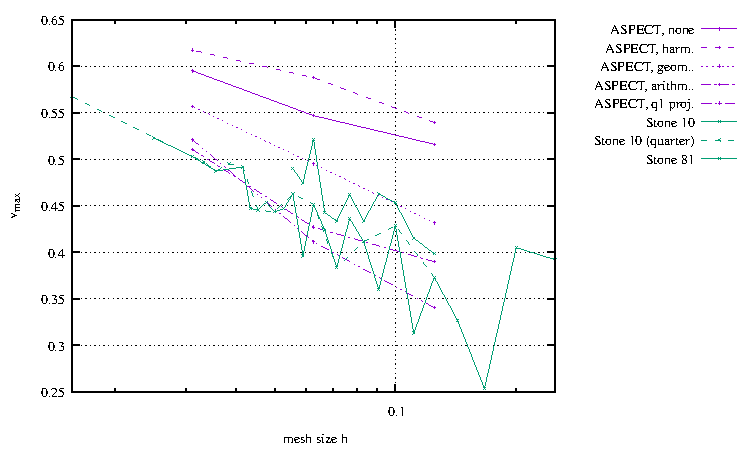
\includegraphics[width=5cm]{images/stokes_sphere3D/max_vel_FS}
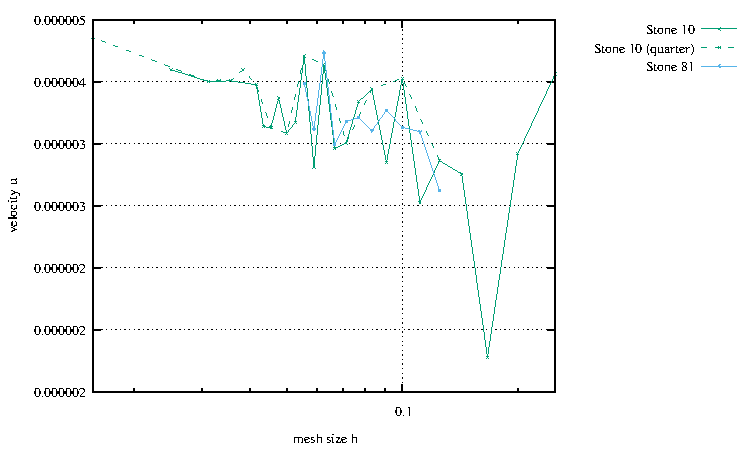
\includegraphics[width=5cm]{images/stokes_sphere3D/max_u_FS}\\
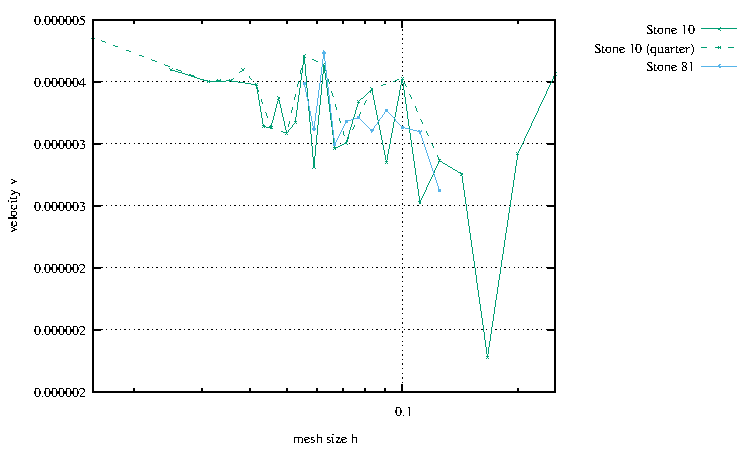
\includegraphics[width=5cm]{images/stokes_sphere3D/max_v_FS}
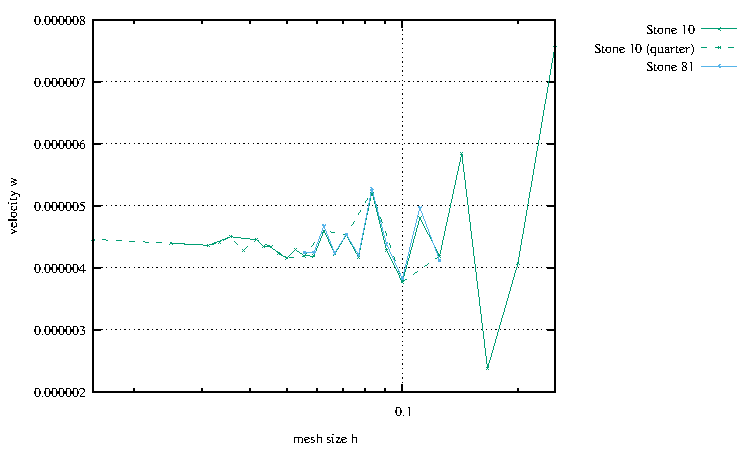
\includegraphics[width=5cm]{images/stokes_sphere3D/max_w_FS}
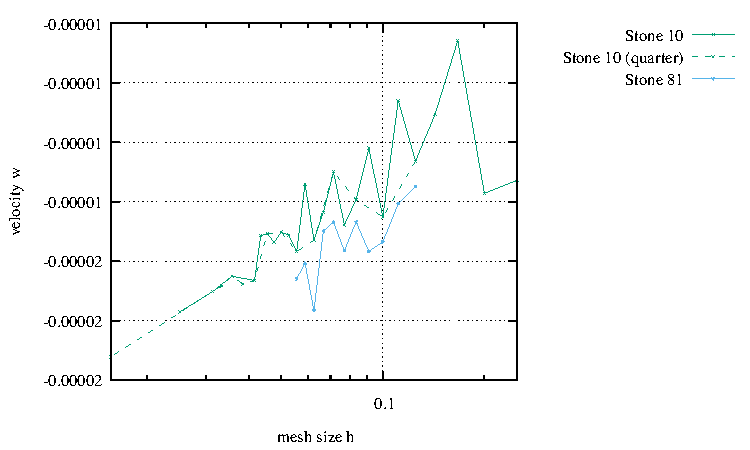
\includegraphics[width=5cm]{images/stokes_sphere3D/min_w_FS}\\
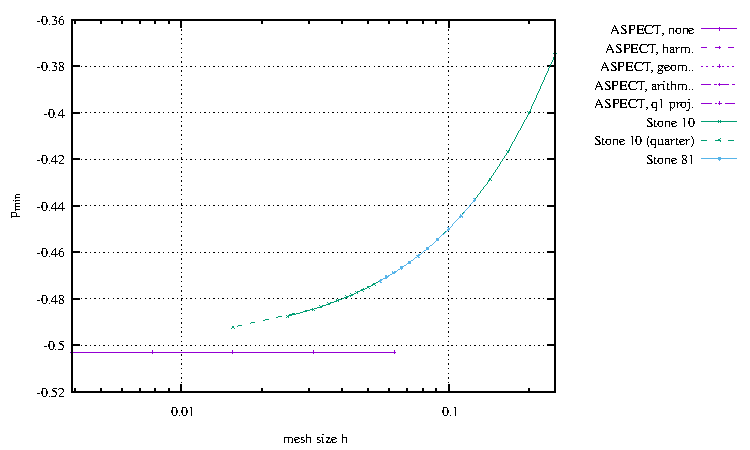
\includegraphics[width=5cm]{images/stokes_sphere3D/pressure_min_FS}
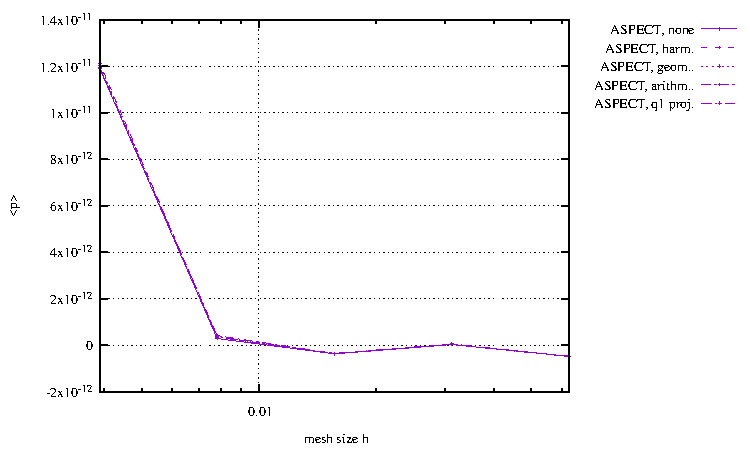
\includegraphics[width=5cm]{images/stokes_sphere3D/pressure_mean_FS}
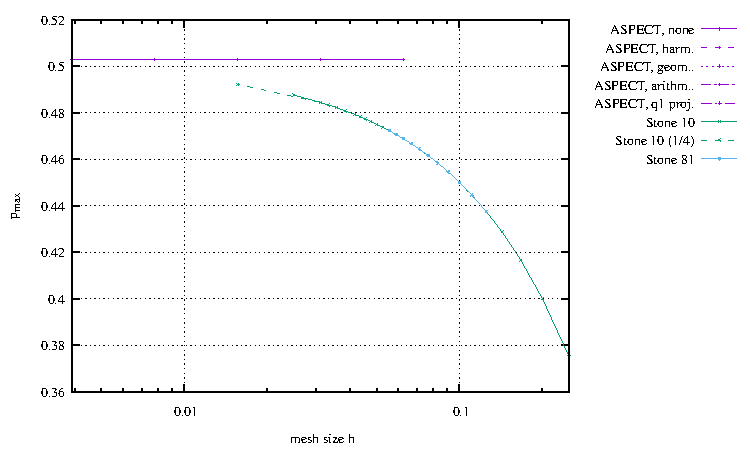
\includegraphics[width=5cm]{images/stokes_sphere3D/pressure_max_FS}\\
{\captionfont Measurements obtained with \aspect and \stone 10 for various averaging schemes.}
\end{center}

\begin{center}
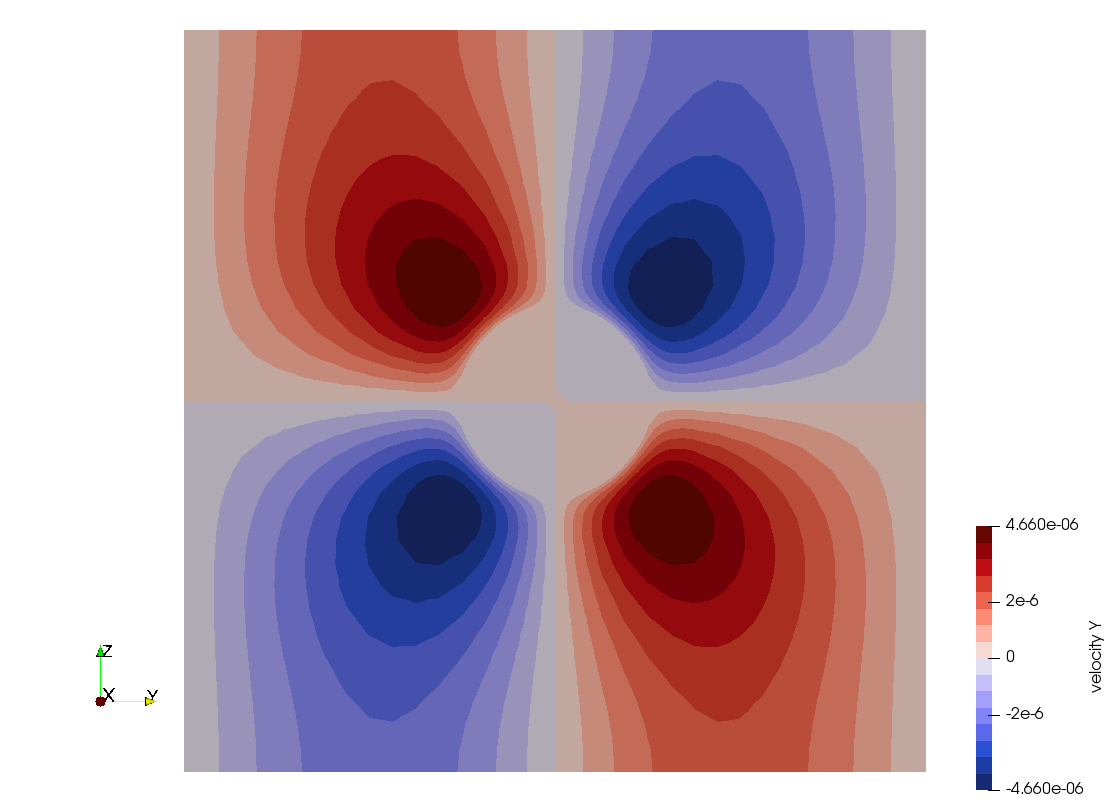
\includegraphics[width=5cm]{images/stokes_sphere3D/aspect_amr_FS/vely}
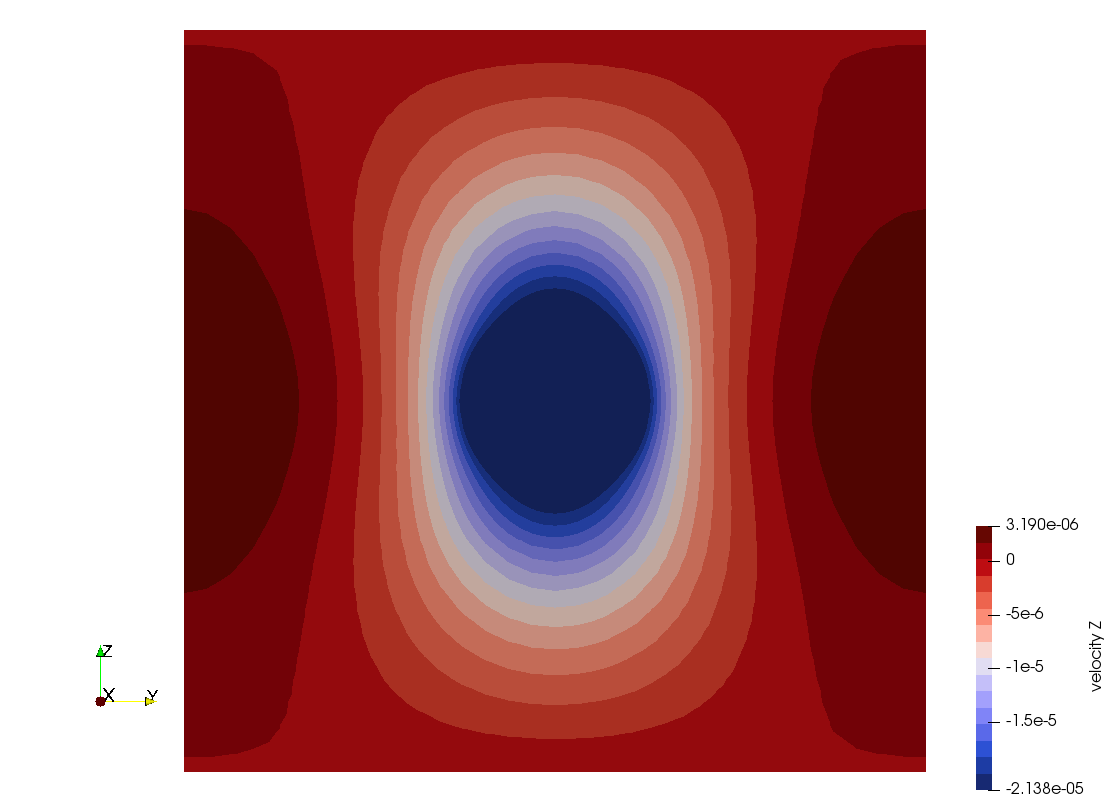
\includegraphics[width=5cm]{images/stokes_sphere3D/aspect_amr_FS/velz}
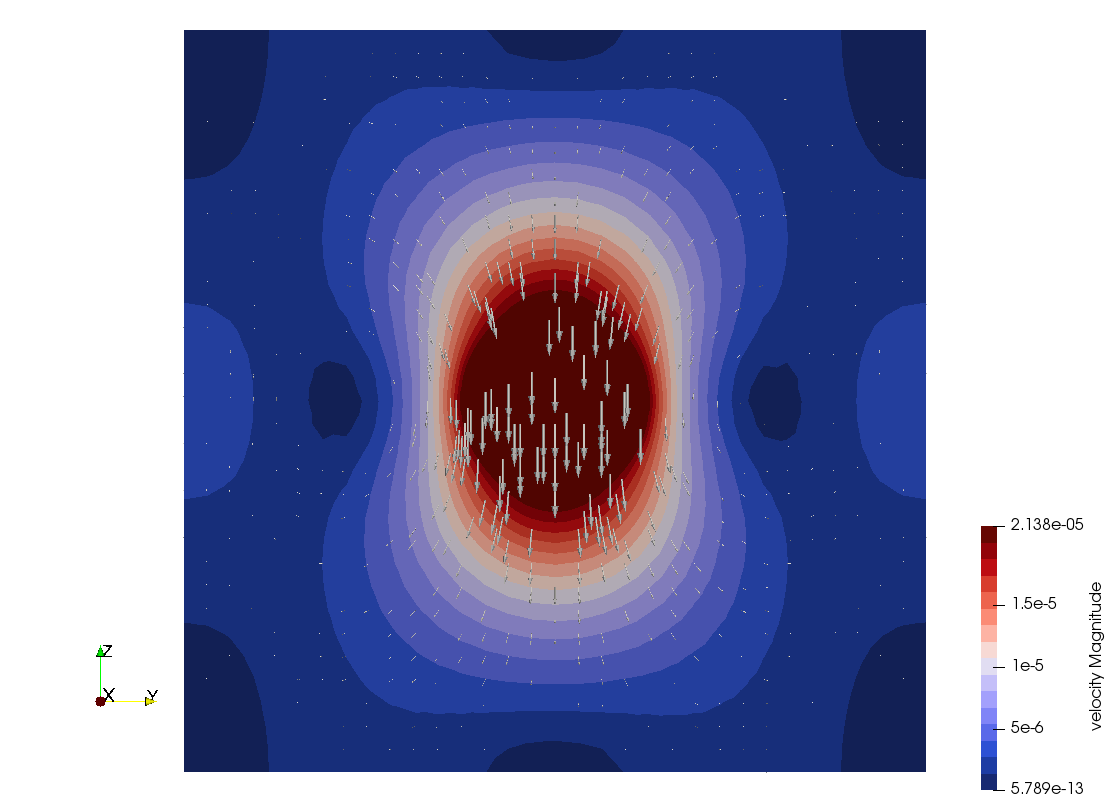
\includegraphics[width=5cm]{images/stokes_sphere3D/aspect_amr_FS/vel}\\
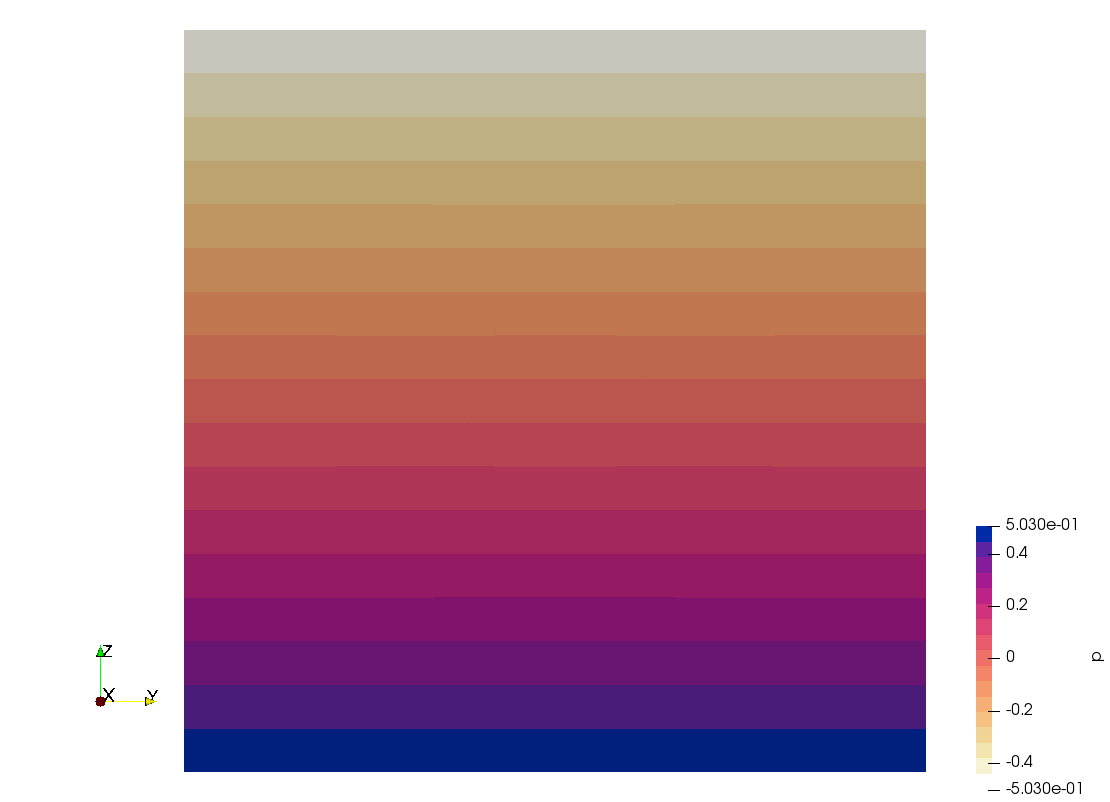
\includegraphics[width=5cm]{images/stokes_sphere3D/aspect_amr_FS/press}
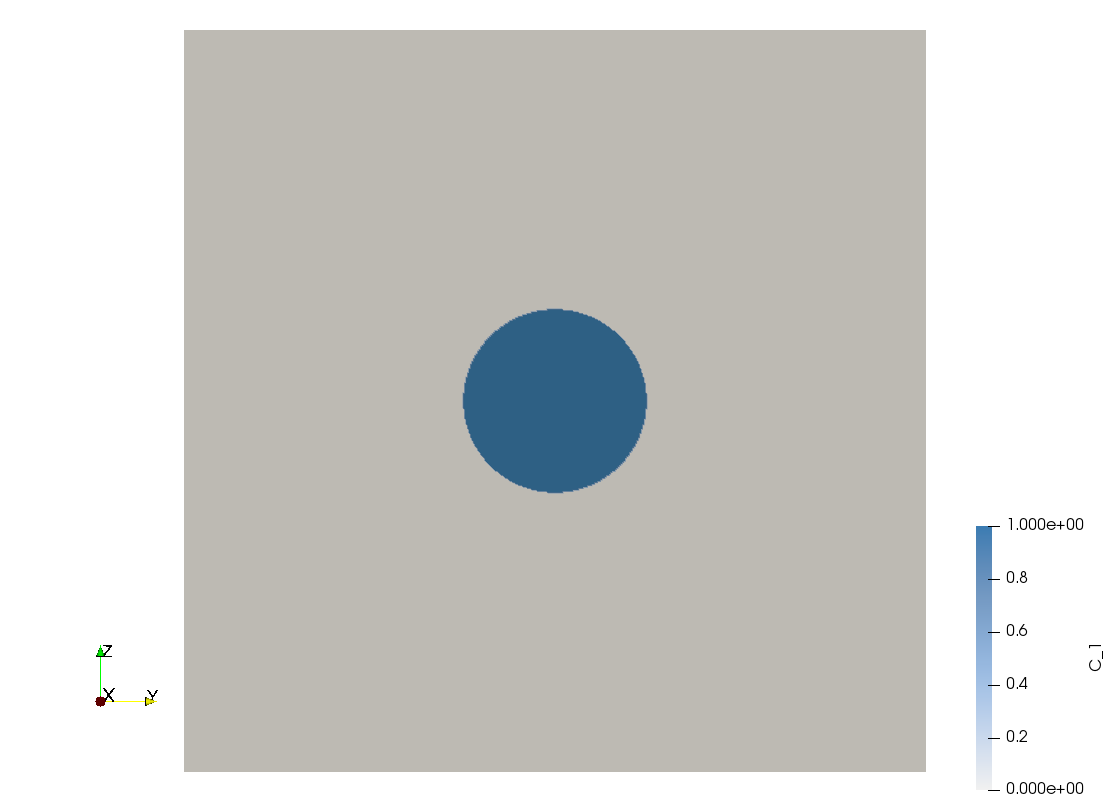
\includegraphics[width=5cm]{images/stokes_sphere3D/aspect_amr_FS/C1}\\
{\captionfont High-resolution solution cross section at $x=0.5$}
\end{center}

\newpage
%.................................................................................
\paragraph{NS results}

\begin{center}
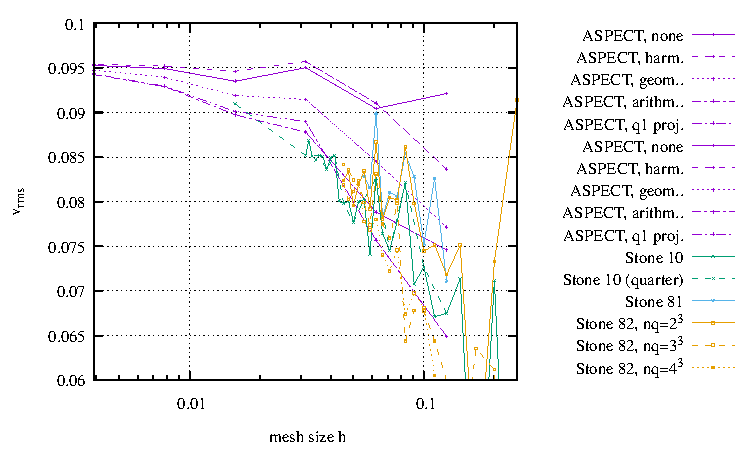
\includegraphics[width=5cm]{images/stokes_sphere3D/vrms_NS}
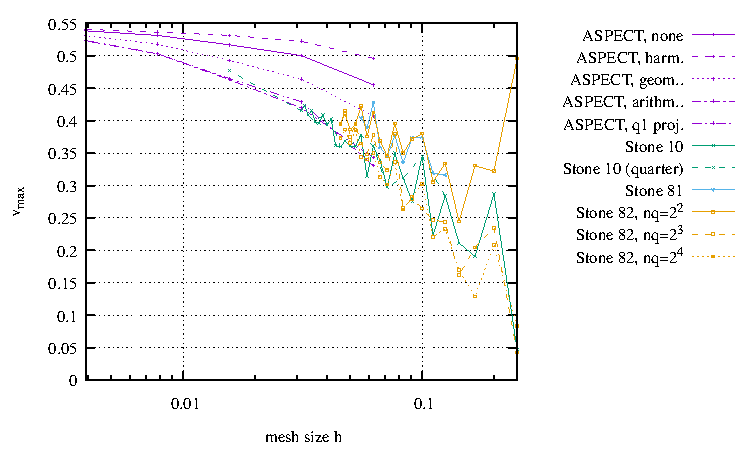
\includegraphics[width=5cm]{images/stokes_sphere3D/max_vel_NS}
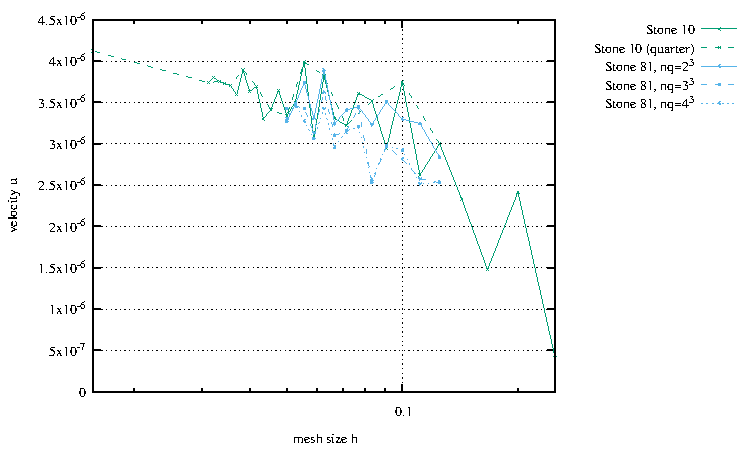
\includegraphics[width=5cm]{images/stokes_sphere3D/max_u_NS}\\
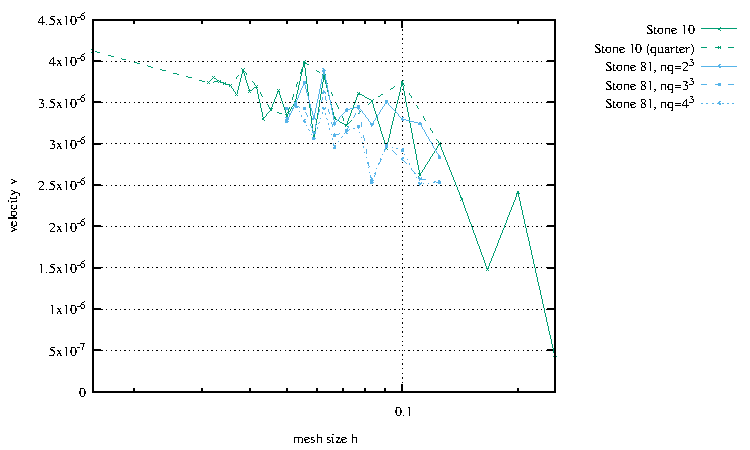
\includegraphics[width=5cm]{images/stokes_sphere3D/max_v_NS}
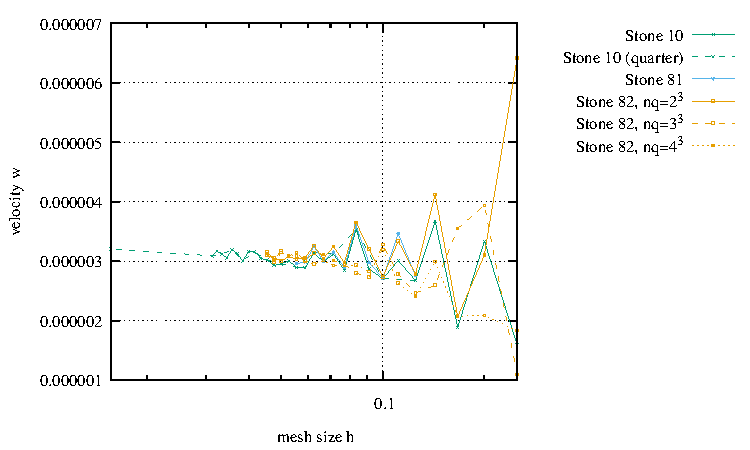
\includegraphics[width=5cm]{images/stokes_sphere3D/max_w_NS}
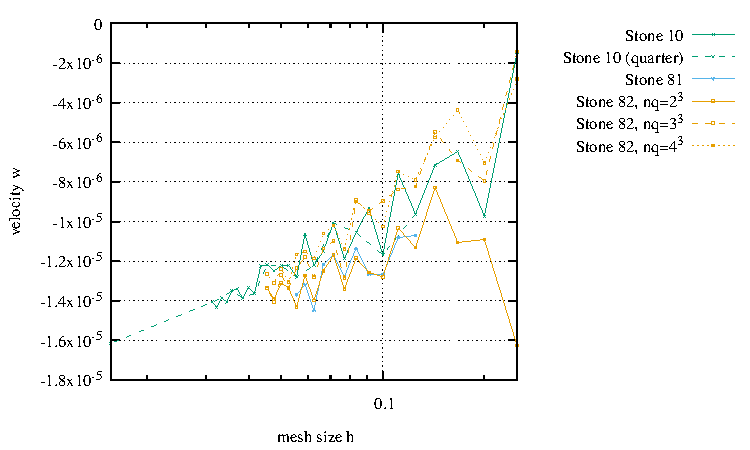
\includegraphics[width=5cm]{images/stokes_sphere3D/min_w_NS}\\
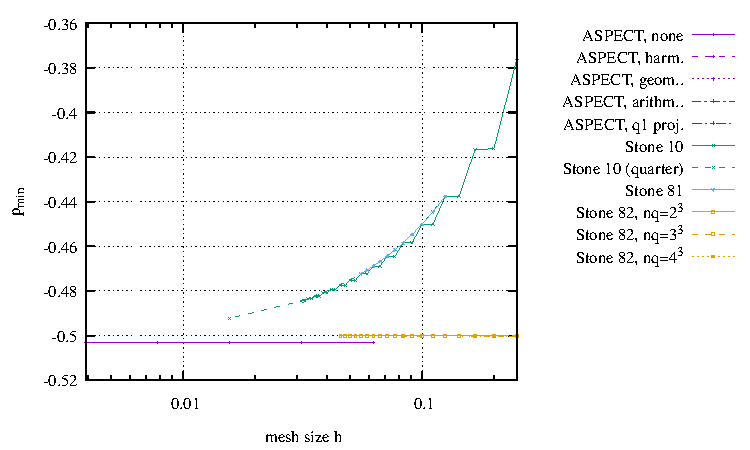
\includegraphics[width=5cm]{images/stokes_sphere3D/pressure_min_NS}
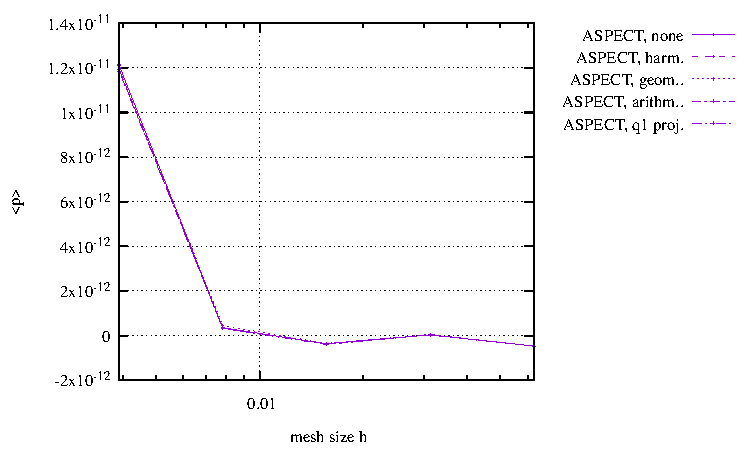
\includegraphics[width=5cm]{images/stokes_sphere3D/pressure_mean_NS}
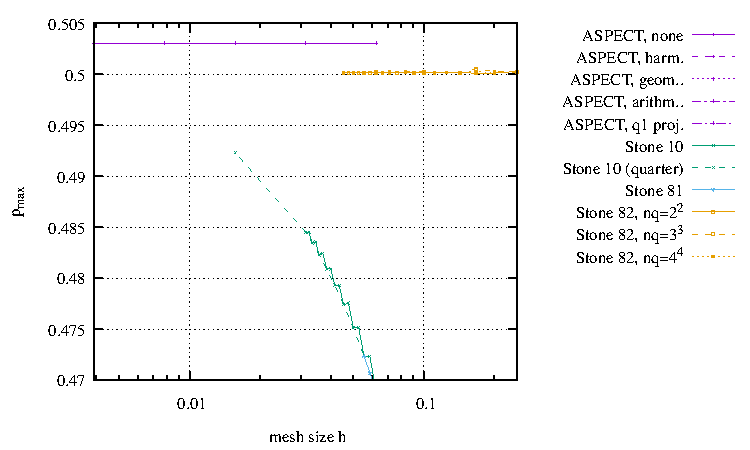
\includegraphics[width=5cm]{images/stokes_sphere3D/pressure_max_NS}\\
{\captionfont Measurements obtained with \aspect and \stone 10 for various averaging schemes.}
\end{center}

\begin{center}
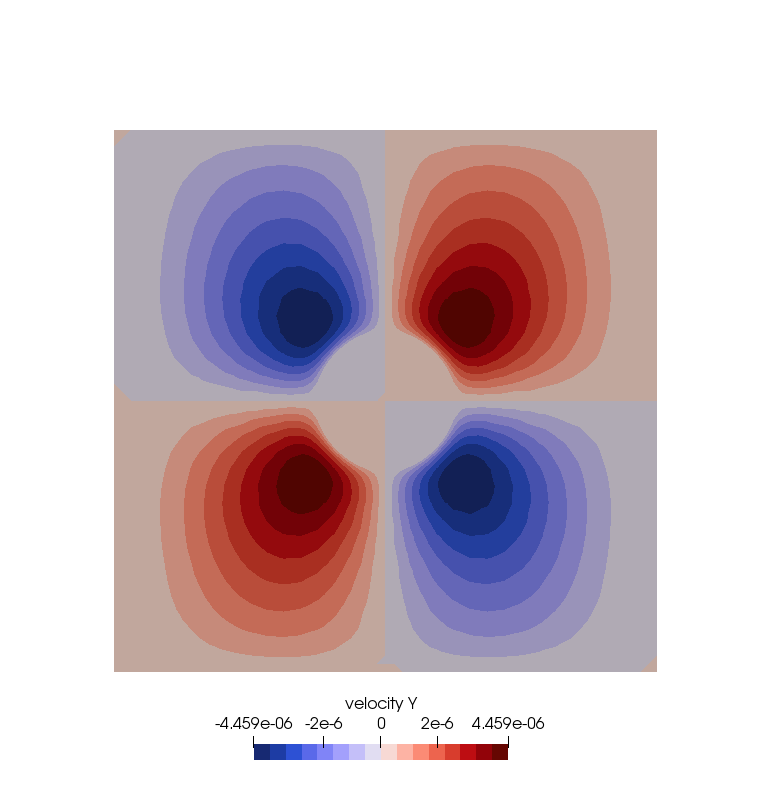
\includegraphics[width=5cm]{images/stokes_sphere3D/aspect_amr_NS/v}
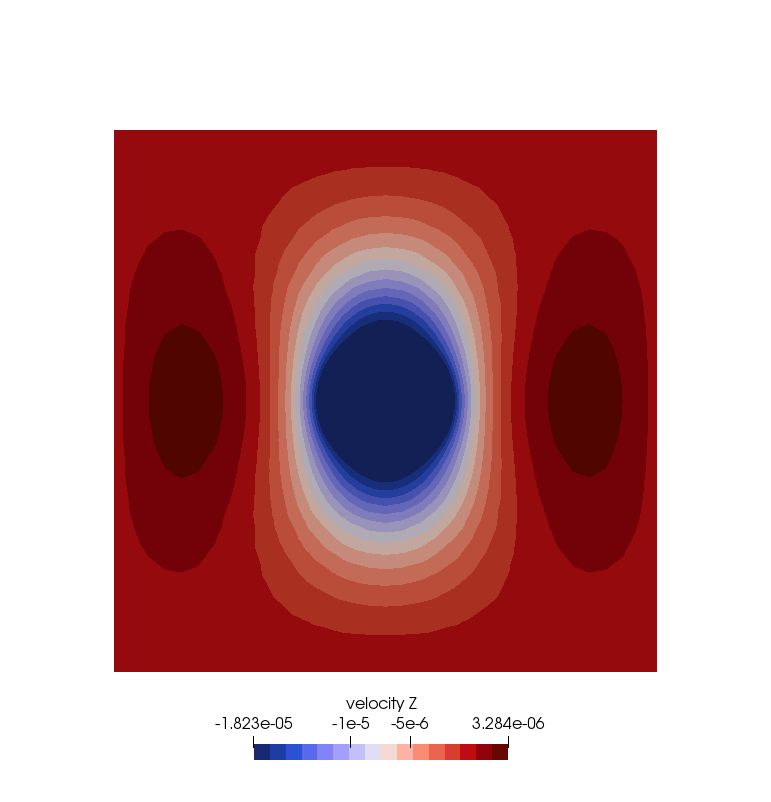
\includegraphics[width=5cm]{images/stokes_sphere3D/aspect_amr_NS/w}
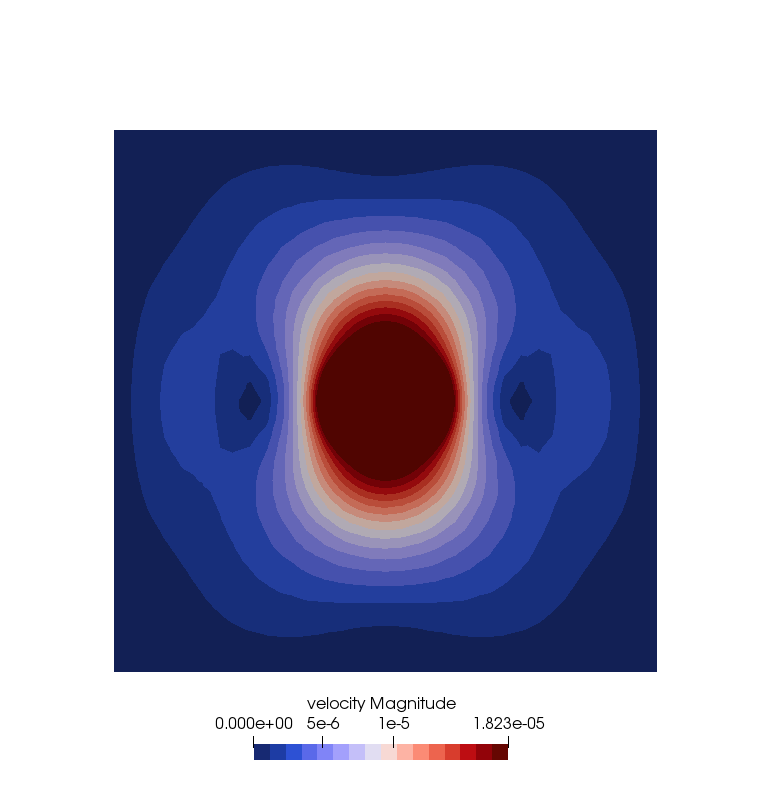
\includegraphics[width=5cm]{images/stokes_sphere3D/aspect_amr_NS/vel}
{\captionfont 4+4 mesh}
\end{center}



\newpage
%.................................................................................
\paragraph{OT results}

\begin{center}
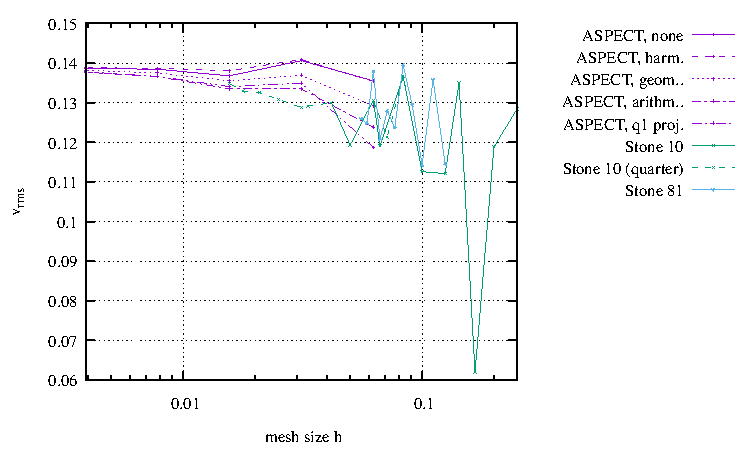
\includegraphics[width=5cm]{images/stokes_sphere3D/vrms_OT}
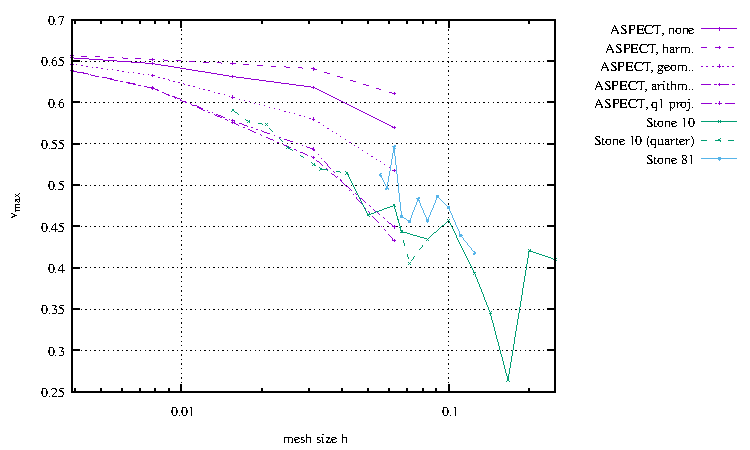
\includegraphics[width=5cm]{images/stokes_sphere3D/max_vel_OT}
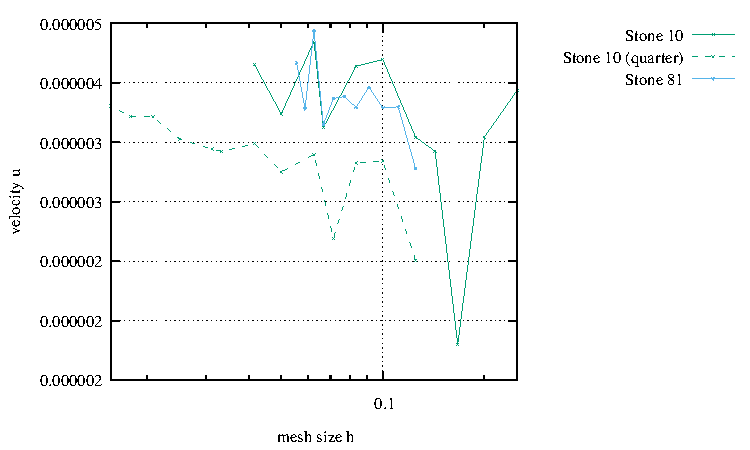
\includegraphics[width=5cm]{images/stokes_sphere3D/max_u_OT}\\
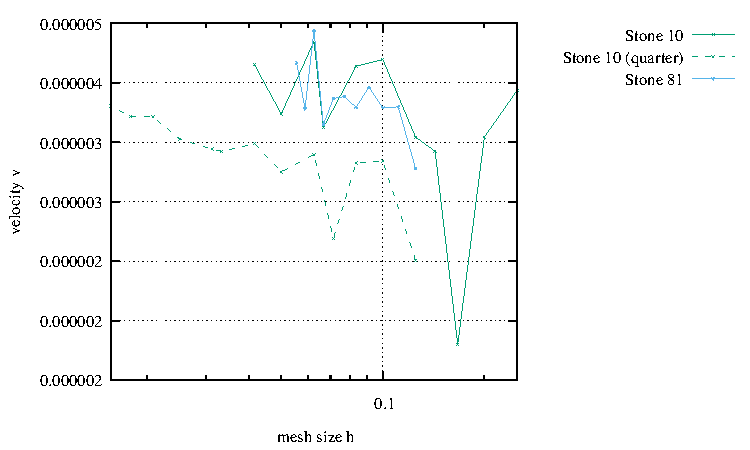
\includegraphics[width=5cm]{images/stokes_sphere3D/max_v_OT}
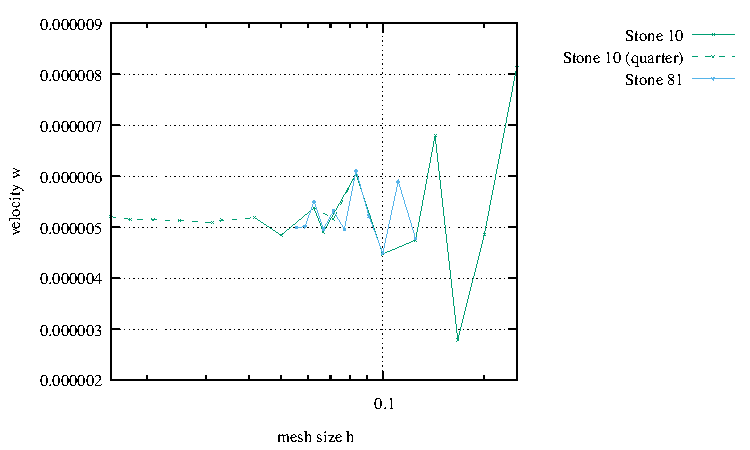
\includegraphics[width=5cm]{images/stokes_sphere3D/max_w_OT}
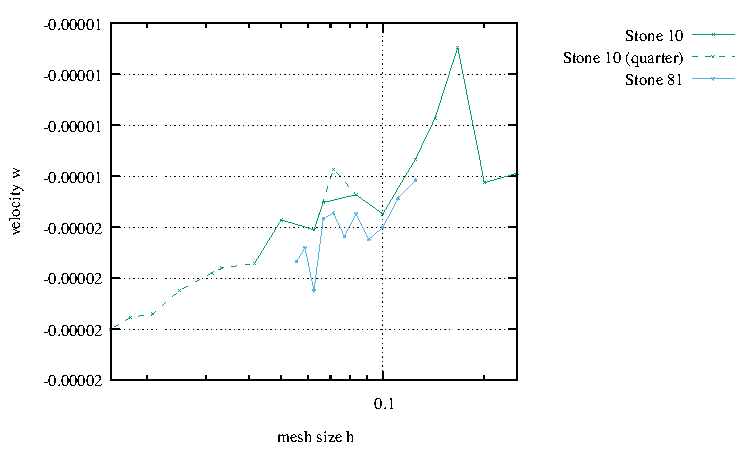
\includegraphics[width=5cm]{images/stokes_sphere3D/min_w_OT}\\
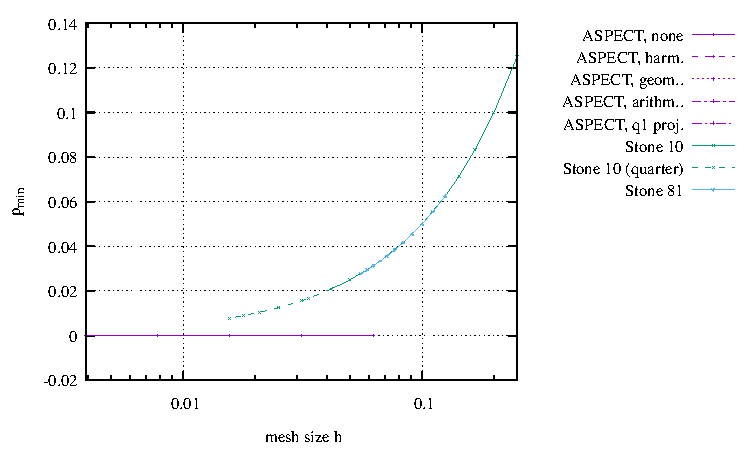
\includegraphics[width=5cm]{images/stokes_sphere3D/pressure_min_OT}
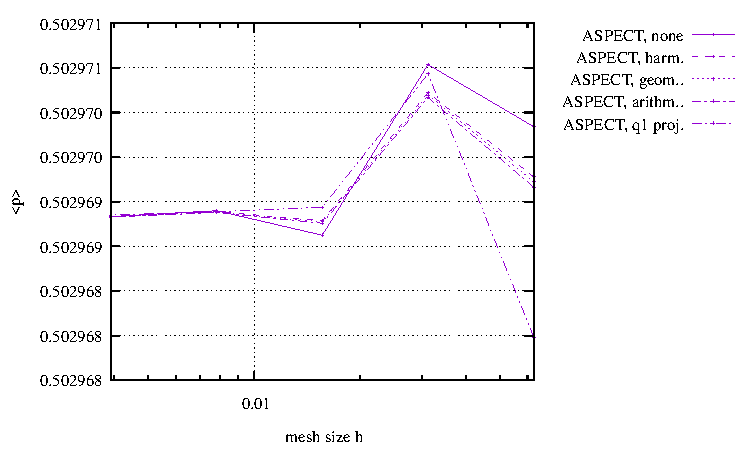
\includegraphics[width=5cm]{images/stokes_sphere3D/pressure_mean_OT}
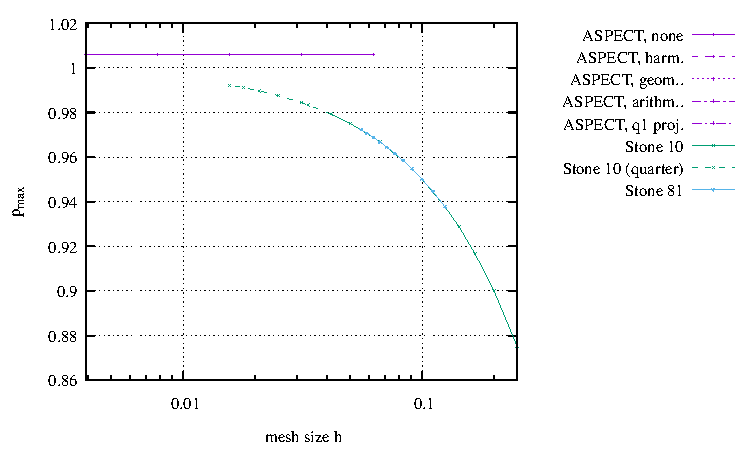
\includegraphics[width=5cm]{images/stokes_sphere3D/pressure_max_OT}\\
{\captionfont Measurements obtained with \aspect and \stone 10 for various averaging schemes.}
\end{center}


\begin{center}
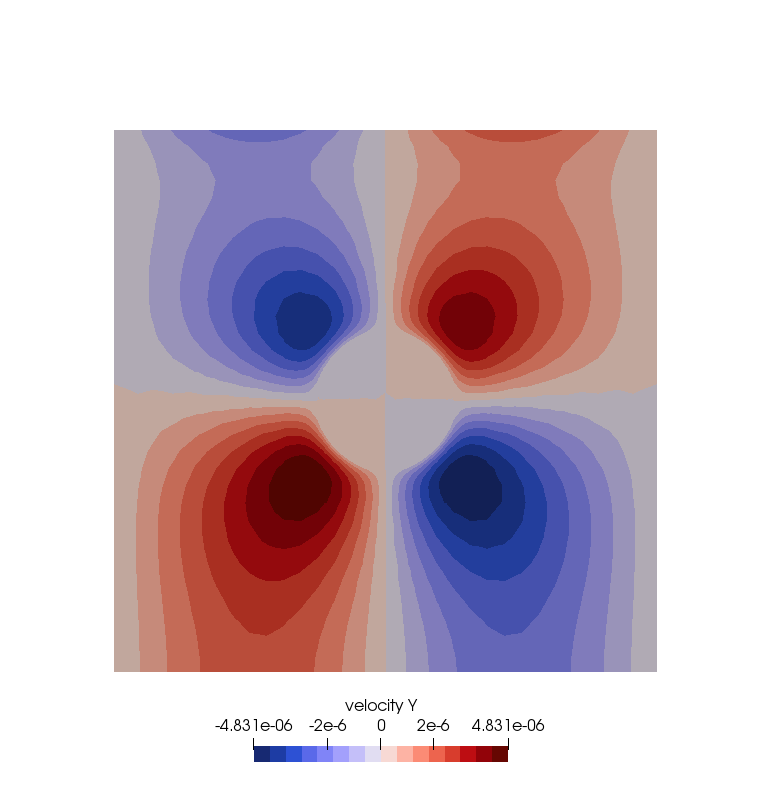
\includegraphics[width=5cm]{images/stokes_sphere3D/aspect_amr_OT/v}
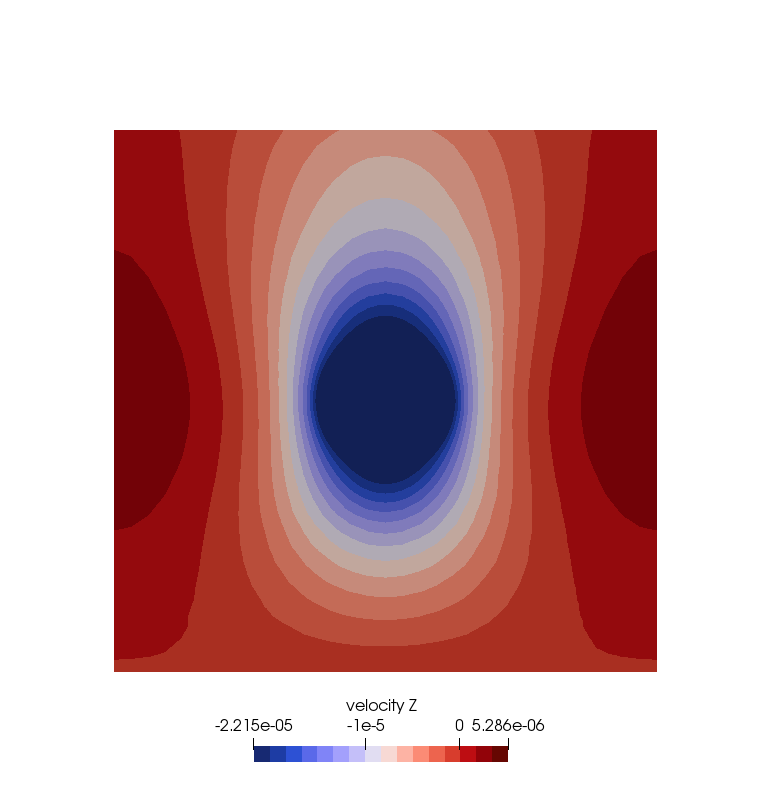
\includegraphics[width=5cm]{images/stokes_sphere3D/aspect_amr_OT/w}
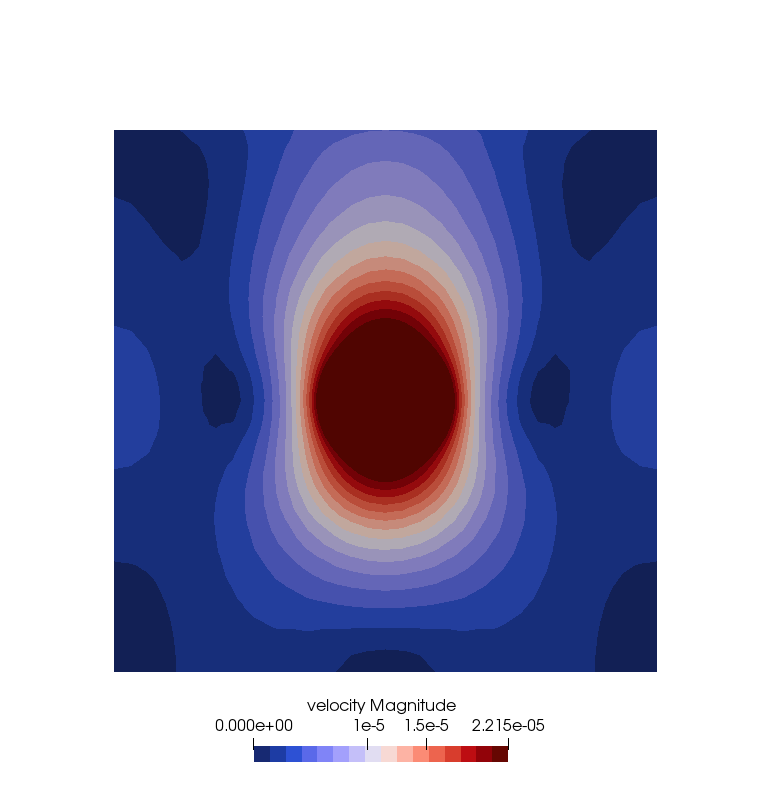
\includegraphics[width=5cm]{images/stokes_sphere3D/aspect_amr_OT/vel}
{\captionfont 4+4 mesh}
\end{center}

\newpage
%.................................................................................
\paragraph{CYL results}.

note that sphere and walls are only 1000 times more viscous than fluid

\begin{center}
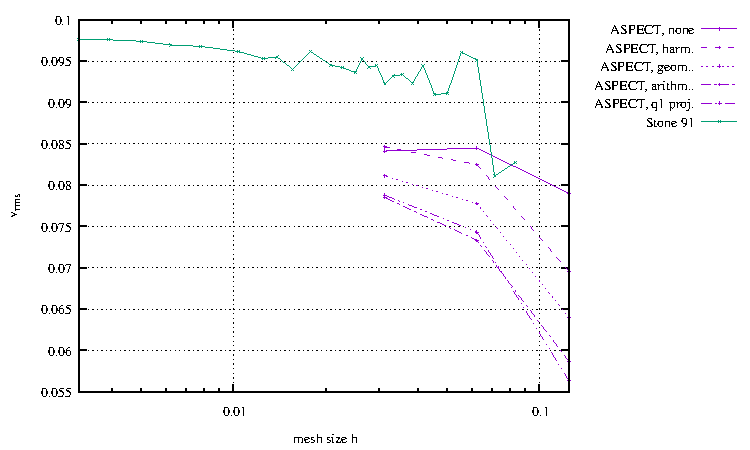
\includegraphics[width=5cm]{images/stokes_sphere3D/vrms_CYL}
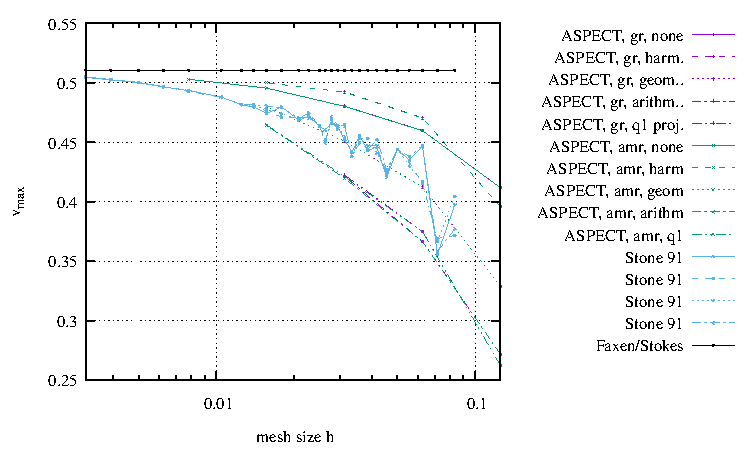
\includegraphics[width=5cm]{images/stokes_sphere3D/max_vel_CYL}
\end{center}

\begin{center}
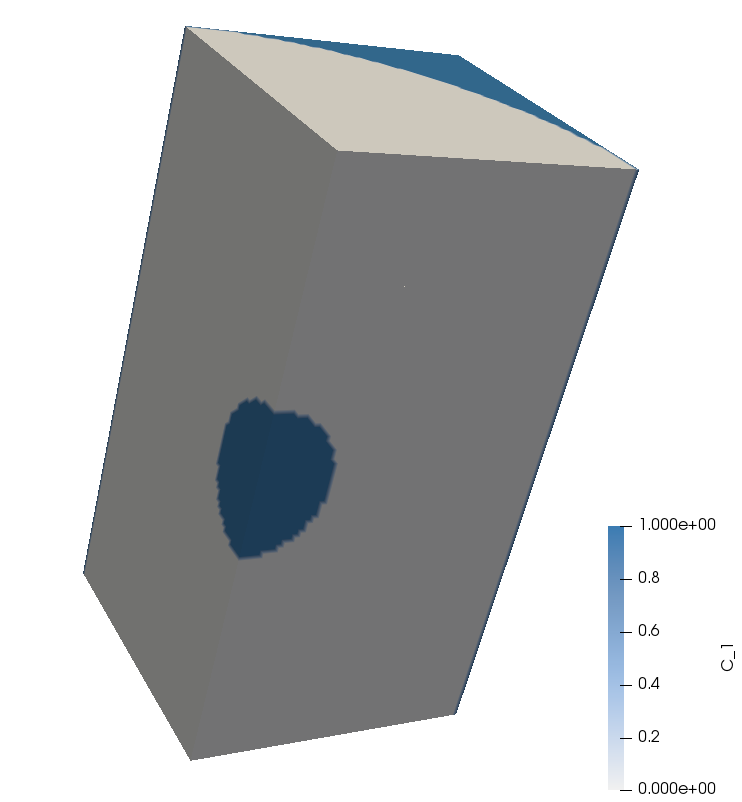
\includegraphics[width=4cm]{images/stokes_sphere3D/aspect_gr_CYL/C1a}
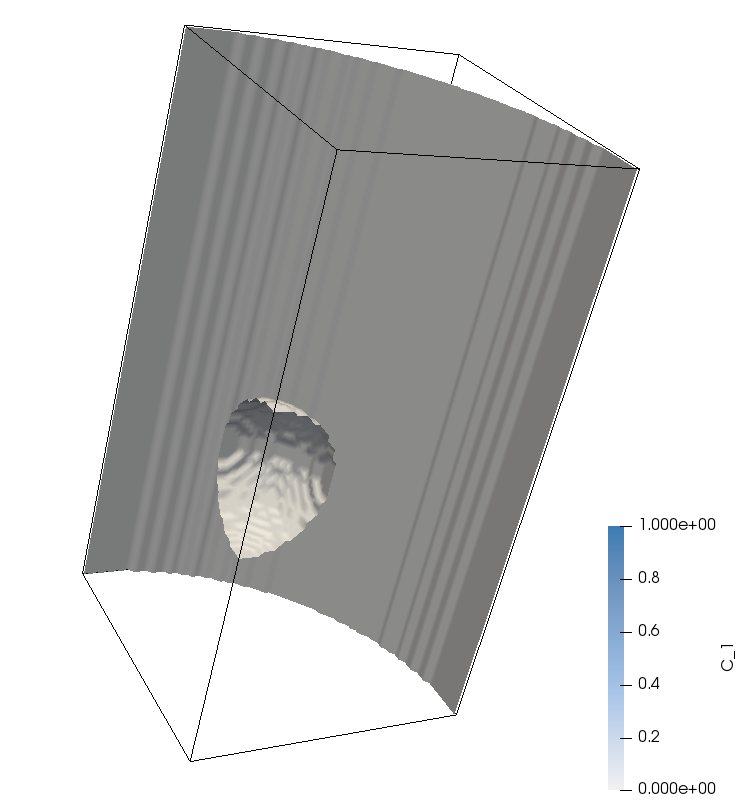
\includegraphics[width=4cm]{images/stokes_sphere3D/aspect_gr_CYL/C1b}
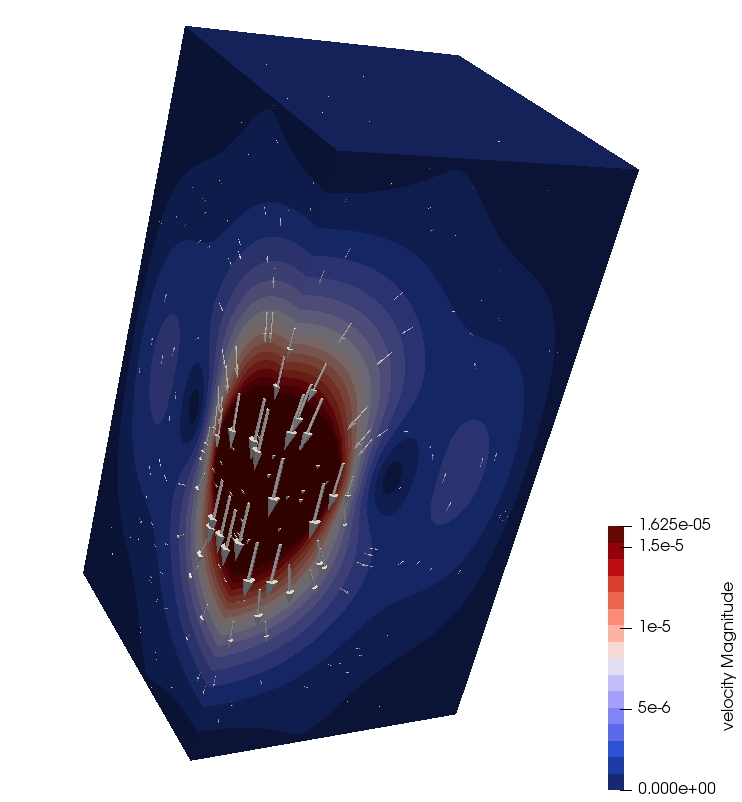
\includegraphics[width=4cm]{images/stokes_sphere3D/aspect_gr_CYL/vel}\\
\includegraphics[width=4cm]{images/stokes_sphere3D/aspect_gr_CYL/u}
\includegraphics[width=4cm]{images/stokes_sphere3D/aspect_gr_CYL/v}
\includegraphics[width=4cm]{images/stokes_sphere3D/aspect_gr_CYL/w}\\
\includegraphics[width=4cm]{images/stokes_sphere3D/aspect_gr_CYL/sr}
\includegraphics[width=4cm]{images/stokes_sphere3D/aspect_gr_CYL/press}\\
{\captionfont level 5 mesh, 32x32x64 elements.}
\end{center}

I have proven in \stone 92 that the sphere should probably be $10^6$
times more viscous than the fluid and the box should be 1.5 in height 
to recover the Habermann/Faxen velocities. 

\begin{center}
\includegraphics[width=4cm]{images/stokes_sphere3D/aspect_amr_CYL/C1_0}
\includegraphics[width=4cm]{images/stokes_sphere3D/aspect_amr_CYL/C1_1}
\includegraphics[width=4cm]{images/stokes_sphere3D/aspect_amr_CYL/C1_2}
\includegraphics[width=4cm]{images/stokes_sphere3D/aspect_amr_CYL/C1_3}
\end{center}



